\chapter{Wärmeleitungsproblem}
\label{cha:2}

\section{Herleitung der Wärmeleitungsgleichung}

Im Allgemeinen beschreibt die Wärmegleichung die Ausbreitung der Wärme in einem Medium. Das Medium kann beispielsweise ein räumlicher Gegenstand sein, zum Beispiel eine rechteckige Metallplatte. Man stelle sich vor, die gegebene Platte wird in der Mitte kurz erhitzt. Diesen Prozess kann man mithilfe einer Wärmebildkamera sichtbar machen.\\

Würde man diese Situation über einen Zeitraum beobachten, so würde man feststellen, dass die Temperatur in der Mitte der Platte sich über die gesamte Fläche verteilt. Und irgendwann kommt es zum Abkühlen, also zur Gleichverteilung der Temperatur in der Platte.\\

Der beschriebene Prozess kann mithilfe sogenannter Wärmeleitungsgleichung modelliert werden, die wir zunächst herleiten möchten.

\subsubsection*{Wärmeausbreitung}
Sei $\Omega \subset \R^{3}$ das Gebiet auf dem die Verteilung der Temperatur bestimmt werden soll.\footnote{\label{foot:1.2.1} Im Allgemeinen gilt $\Omega \subset \R^n$.} Die gesuchte Temperaturverteilung auf $\Omega$ in einem Zeitintervall $T = [t_0, t_1] \subset \R$ bezeichnen wir mit $u$. $u$ ordnet jedem Punkt $x \in \Omega$ zu jedem Zeitpunkt $t \in T$ eine Zahl $u(x, t) \in \R$ zu, also $u:\Omega \times T \longrightarrow \R$. Zusätzlich wollen wir die Bewegung der Wärme in $\Omega$ auffassen, es ist der Wärmefluss $j$. Für jeden Punkt $x \in \Omega$ zu jedem Zeitpunkt $t \in T$ gibt der Wärmefluss die Richtung in der die Wärmeenergie transportiert wird an, somit $j:\Omega \times T \longrightarrow \R^3$. Damit sind nötigen \textit{Variablen} für die Modellierung festgelegt.\\

Für die Herleitung der Gleichungen der Modellierung wird ein beliebiges Volumen $V \subset \Omega$ betrachtet. In einem homogenen Fall, also es gibt keine Wärmequellen, die in das Volumen $V$ die Wärmeenergie hinein oder heraus transportieren, würde man keinen Wärmestrom am Rand $dV$ detektieren, es gilt also

\begin{eqnarray}
	\int\limits_{\partial V} \langle j, v \rangle dS = 0.
	\label{equa:2.1_1}
\end{eqnarray}

Mit der Gleichung \ref{equa:2.1_1} wird der Strom $j$ in Richtung jeder Normalen $v$ am Rand $dV$ von $V$ aufsummiert (Abb.\ref{fig:1.2_1}). Und mit der Annahme, dass es keine Quellen gibt, erwarten wir eine 0 Summe.

%----------------------------------------------------------------------------------------
%	Beginn der Grafik
%----------------------------------------------------------------------------------------
\begin{figure}[!h]
	\centering
	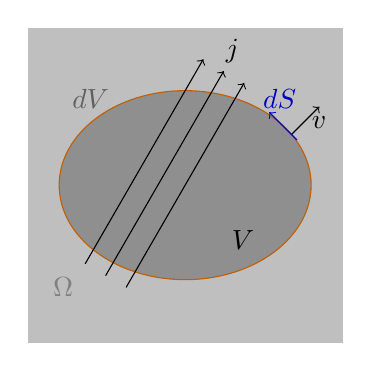
\begin{tikzpicture}
		
		
		\fill[lightgray] (0,0) ellipse (1.6cm and 1.2cm);	
		\draw[orange] (0,0) ellipse (1.6cm and 1.2cm);
		\draw[black](1, -0.7) node [left] {$V$};
		
		\draw [rotate=-30, xshift=-0.6cm, yshift=0.5cm, ->] [black] (0,-2) -- (0,1); % j
		\draw [rotate=-30, xshift=-0.3cm, yshift=0.5cm, ->] [black] (0,-2) -- (0,1); % j
		\draw [rotate=-30, xshift=0cm, yshift=0.5cm, ->] [black] (0,-2) -- (0,1); % j
		\draw [black] (0.6, 1.7)  node {$j$};	
		
		\draw [rotate=-45, xshift=0.5cm, yshift=1.41cm, ->] [black] (0,0) -- (0,0.5); % v
		\draw [black] (1.7,0.8)  node {$v$};	
		\draw [rotate=45, xshift=1.41cm, yshift=-0.6cm, ->] [blue] (0,0) -- (0,0.5); % dS
		\draw [blue] (1.2, 1.1)  node {$dS$};

		\draw [gray] (-1.2, 1.1)  node {$dV$};
						
		\fill[nearly transparent] (-2,-2) rectangle (2, 2); // Omega
		\draw[gray](-1.3, -1.3) node [left] {$\Omega$};
		
	\end{tikzpicture}	
	\caption{Schematische Darstellung der Gleichung \ref{equa:2.1_1}, mit $V$ das Volumen eine Mediums, $dV$ Rand (orange) von $V$, $j$ Der Wärmestrom durch $V$, $v \in \R^3$ Normalenvektor an $dV$ und $dS$ Tangente an $dV$.}
	\label{fig:1.2_1}
\end{figure}
%----------------------------------------------------------------------------------------
%	Ende der Grafik
%----------------------------------------------------------------------------------------

An dieser Stelle benötigen wie den \textit{Gauß'schen Satz} um das Oberflächenintegral \ref{equa:2.1_1} in ein Volumenintegral umzuschreiben.

\begin{Definition}
	\textbf{Der Gauß'sche Satz} \\
	Sei $V \subset	\R^n$ kompakt mit abschnittsweise glattem Rand $S = \partial V$, der Rand ist orientiert durch äußeres Normaleneinheitsvektorfeld $n$. Das Vektorfeld $F$ sei stetig differenzierbar auf einer offenen Menge $\Omega$ mit $V \in \Omega$. Dann gilt
	\begin{equation}
		\int\limits_{V} \langle \nabla,F \rangle dV = \int\limits_{\partial V} \langle F,n \rangle
		 dS.
		 \label{fig:2.1_2}
	\end{equation}
\end{Definition}

\begin{framed}
	\paragraph{Temporäres DenkZettel}

	\begin{itemize}
		\item[] \begin{Definition}
			Kompakte Menge \\
			$\R^n$ ist metrischer Raum. Wenn es für jede \textbf{offene Überdeckung} von $A \subset \R^n$, eine endliche Überdeckung gibt, also 
			\begin{eqnarray*}
				A \subset \bigcup\limits_{i \in I} U_i, \ \ \mbox{mit endlichem} \ I
			\end{eqnarray*} 			
		\end{Definition}
		\item[] \begin{Definition}
			Glatter Rand \\
			Sei $A \in \R^n$ kompakt, $A$ hat einen glatten Rand, wenn es zu jeden Punkt $x \in \partial A$ eine offene Umgebung $U \subseteq \R^n$ und $\psi : U \rightarrow \R, \ \psi \in C^n$ so gibt, dass 
			\begin{itemize}
				\item [(a)] $A \cap U = \{x \in U : \ \psi(x) \leq 0 \}$ 
				\item [(b)] $\forall x \in U : \psi'(x) \neq 0$
			\end{itemize}
			gilt.
		\end{Definition}		
	\end{itemize}
\end{framed}

Nun, der Gauß'sche Satz angewandt auf Gleichung \ref{equa:2.1_1} liefert folgendes Ergebnis
\begin{eqnarray}
	\int\limits_{V} \langle \nabla, j \rangle dx = \int\limits_{\partial V} \langle j, v \rangle dS = 0
	\label{fig:2.1_3}
\end{eqnarray}
Da, das Volumen $V$ nicht näher spezifiziert war, können wir aus \ref{fig:2.1_3} folgern, dass
{\color{red} Dahmen/Reusken: S.456, sinnvolle Argumentation nach dem Gaußschen Satz} \\

\begin{eqnarray}
	\langle \nabla, j \rangle = 0
	\label{equa:2.1_4}
\end{eqnarray}
auf ganz $\Omega$ gilt.

Als Nächstes, wollen wir herausfinden, wie $j$ und $u$ von einander abhängen. Eine einfache Modellannahme gibt uns das \textit{Fourier'sche Gesetz}:\footnote{\label{foot:1.2.2} J. B. Fourier, 1768-1830} 

\begin{center}
	\begin{minipage}{0.8\textwidth}
		\textit{Die Wärmeenergie strömt immer von Wärmeren Regionen zu den kälteren. Die Flussrate des Stroms ist proportional zum Temperaturgradienten.}
	\end{minipage}
\end{center}

Eine weitere Annahme für das Modell ist, dass jedes Material eine Eigenschaft hat, die Wärme auf seine Art und Weise zu leiten. Diese Eigenschaft nennt man die \textit{Wärmeleitfähigkeit} $a$. Sie ordnet jedem Punkt im Körper eine positive Zahl zu, also $a: \Omega \rightarrow \R_+$. Führen wir beide Überlegungen zusammen und erhalten 
\begin{eqnarray}
	j = -a \nabla u.
	\label{equa:2.1_5}
\end{eqnarray}
Einsetzen der Gleichung \ref{equa:2.1_5} in \ref{equa:2.1_4} führt uns zum folgenden Ausdruck
\begin{eqnarray}
	-\langle \nabla, a \nabla u \rangle = 0
	\label{equa:2.1_6}
\end{eqnarray}
Falls auf $\Omega$ noch zusätzliche Wärmequellen $f:\Omega \rightarrow \R$ vorhanden sind und die Wärmeverteilung \textit{instationär} ist, erhalten wir insgesamt folgende Gleichung \cite[S.5]{Schweizer18}
\begin{eqnarray}
	c \rho \ \partial_t u - \langle \nabla, a\nabla u \rangle = f
	\label{equa:2.1_7}
\end{eqnarray}

$c$ spezifische Wärmekapazität $[J/Kkg]$ \\
$\rho$ - Einheit $[kg/m^3]$ \\


{\color{red} Einschub über die Klassifikation der DGL} \\

Nie Gleichung \ref{equa:2.1_7} beschreibt ein abstraktes System. Die sogenannten Anfangs- und Randbedingungen würden eine mehr der Realität entsprechende Beschreibung des Wärmeleitungsproblems liefern. Jedes physikalische System besitzt zum Anfang der Messung oder der Beobachtung einen gewissen Anfangszustand $u_0$. Meistens wird die Zeit $t$ zu diesem Anfang auf den Wert 0 gesetzt, somit erhalten wir

\begin{eqnarray}
	u(x,0) = u_0(x), \ x \in \Omega
	\label{equa:2.1_8}
\end{eqnarray}

Die Randbedingungen geben die Temperaturverteilung $u$ am Rand $\partial \Omega$ des Gebiets $\Omega$ und können im Allgemeinen mit Sturm'schen Randbedingungen angegeben werden ({\color{red} oder gemischte Randbedingung?}):

\begin{eqnarray}
	u(x,t) = g(x, t), \ x \in \partial \Omega 
	%\dfrac{\partial}{\partial v} u(x,t) = \alpha(x)[u(x,t) - g(x)], 
	\label{equa:2.1_9}
\end{eqnarray}   

Nun kann man die Gleichungen \ref{equa:2.1_7}, \ref{equa:2.1_8} und \ref{equa:2.1_9} zusammen in einer Rand- und Anfangswertaufgabe (RAWP) der Wärmeleitung zusammenfassen, also:

\begin{Definition}
	\textbf{Rand- und Anfangswertaufgabe der Wärmeleitung} \\
	Sei $\Omega \subset	\R^3$ ein gebiet mit glattem Rand $\partial \Omega$, der Rand ist orientiert durch äußeres Normaleneinheitsvektorfeld $n$. So beschreibt das Modell
	\begin{equation}
		\begin{array}{llll}
			\partial_t u - \langle \nabla, a\nabla u \rangle & = & f & \\
			u(x,0) & = & u_0(x), & \ x \in \Omega \\
				u(x,t) & = & g(x, t), & \ x \in \partial \Omega
		\end{array}
		\label{equa:2.1_10}
	\end{equation}
	die Rand- und Anfangswertaufgabe der Wärmeleitung für alle $t \in T \subset \R$. 
	\label{def:2.1_4}
\end{Definition}

Das Ergebnis dieses Kapitels ist in der obigen Definition \ref{def:2.1_4} angegeben und wird als Grundmodell in folgenden Kapiteln dieser Arbeit vorausgesetzt.  

\subsection{Analytische Untersuchung der Wärmeleitungsgleichung}

Eventuell ...



%=====================================================================================================
% FORWARD PROBLEM 
%=====================================================================================================


\section{Vorwärtsproblem der Wärmeleitungsgleichung}

FEM als Grundlage des numerischen Ansatzes, warum und wieso ...

\subsection{Herleitung der Variationsformulierung der Wärmegleichung}

Die Wärmegleichung lautet:
\begin{equation}
	\partial_t u - \langle \nabla, a\nabla u \rangle  = f,
\end{equation}

und soll in die Variationsformulierung in schwacher Form umgeformt werden:
\begin{equation}
	\int_\Omega \frac{\partial u}{\partial t} v \, dx + \int_\Omega a(u) \nabla u \cdot \nabla v \, dx = \int_\Omega f v \, dx.
\end{equation}

Im Folgenden werden die Schritte zur Herleitung detailliert erläutert.

\subsection{Geometrie und Gitter definieren}
Die Geometrie und das Gitter definieren den Bereich $\Omega$, in dem die Gleichung gelöst wird. Das Gitter teilt diesen Bereich in kleine Unterbereiche (Finite Elemente) auf.

\subsubsection{Warum Geometrie und Gitter definieren?}
\begin{itemize}
	\item Die Methode der Finiten Elemente (FEM) basiert auf der Approximation der Lösung $u(x, y, t)$ auf einer diskreten Darstellung des Gebiets.
	\item Ein Gitter zerlegt $\Omega$ in einfachere Formen (z. B. Dreiecke oder Vierecke). Innerhalb jedes Elements wird die Lösung lokal approximiert.
\end{itemize}

\subsubsection{Beispiel für ein rechteckiges Gebiet}
\begin{equation}
	\Omega = \{(x, y) \mid 0 \leq x \leq L_x, \, 0 \leq y \leq L_y\}.
\end{equation}
Dieses Gebiet könnte mit Dreiecken oder Rechtecken diskretisiert werden.

\subsection{Funktionsräume definieren}
Ein Funktionsraum beschreibt, wie die Lösung $u$ und die Testfunktionen $v$ innerhalb der Finiten Elemente dargestellt werden.

\subsubsection{Was sind $P_1$- und $P_2$-Elemente?}
\begin{itemize}
	\item $P_1$: Lineare Basisfunktionen – $u$ wird innerhalb eines Elements als lineares Polynom approximiert.
	\item $P_2$: Quadratische Basisfunktionen – $u$ wird innerhalb eines Elements als quadratisches Polynom approximiert.
\end{itemize}
Diese Basisfunktionen gewährleisten, dass $u$ über das gesamte Gebiet hinweg stetig ist.

\subsubsection{Warum Funktionsräume definieren?}
Die Funktionsräume sorgen dafür, dass die approximierte Lösung $u$ und die Testfunktionen $v$ die notwendigen Kontinuitäts- und Randbedingungen der PDE erfüllen.

\subsection{Variationsformulierung herleiten}
Die Variationsformulierung (schwache Form) wird durch Multiplikation der PDE mit einer Testfunktion $v$ und Integration über das Gebiet $\Omega$ hergeleitet. Dieser Schritt erlaubt es, auch Lösungen $u$ zu berücksichtigen, die möglicherweise nicht überall differenzierbar sind.

\subsubsection{Herleitung der schwachen Form}
\begin{enumerate}
	\item \textbf{Starte mit der PDE:}
	\begin{equation}
		\frac{\partial u}{\partial t} - \nabla \cdot \big(a(u) \nabla u\big) = f.
	\end{equation}
	
	\item \textbf{Multipliziere mit einer Testfunktion $v$:} Multipliziere beide Seiten mit einer glatten Testfunktion $v \in V$, wobei $V$ der Raum der zulässigen Testfunktionen ist:
	\begin{equation}
		v \left(\frac{\partial u}{\partial t} - \nabla \cdot \big(a(u) \nabla u\big)\right) = v f.
	\end{equation}
	
	\item \textbf{Integriere über $\Omega$:}
	\begin{equation}
		\int_\Omega v \frac{\partial u}{\partial t} \, dx - \int_\Omega v \nabla \cdot \big(a(u) \nabla u\big) \, dx = \int_\Omega v f \, dx.
	\end{equation}
	
	\item \textbf{Wende den Divergenzsatz an:} Für den zweiten Term wende den Divergenzsatz an, um das Volumenintegral in ein Oberflächenintegral umzuwandeln:
	\begin{equation}
		\int_\Omega v \nabla \cdot \big(a(u) \nabla u\big) \, dx = \int_{\partial \Omega} v \big(a(u) \nabla u \cdot \mathbf{n}\big) \, dS - \int_\Omega \nabla v \cdot \big(a(u) \nabla u\big) \, dx.
	\end{equation}
	Hier ist $\partial \Omega$ der Rand des Gebiets und $\mathbf{n}$ der nach außen gerichtete Normalenvektor.
	
	\item \textbf{Vereinfachung bei homogenen Randbedingungen:} Unter der Annahme homogener Dirichlet-Randbedingungen ($u = 0$ auf dem Rand) verschwindet der Oberflächenterm:
	\begin{equation}
		\int_\Omega v \nabla \cdot \big(a(u) \nabla u\big) \, dx = -\int_\Omega \nabla v \cdot \big(a(u) \nabla u\big) \, dx.
	\end{equation}
	
	\item \textbf{Kombiniere die Terme:} Substituiere zurück in die Gleichung. Die schwache Form lautet:
	\begin{equation}
		\int_\Omega v \frac{\partial u}{\partial t} \, dx + \int_\Omega a(u) \nabla u \cdot \nabla v \, dx = \int_\Omega v f \, dx.
	\end{equation}
\end{enumerate}

\subsection{Zeitdiskretisierung}
Die Zeitdiskretisierung ist notwendig, um die Lösung schrittweise für diskrete Zeitpunkte zu berechnen.

\subsubsection{Warum Zeitdiskretisierung?}
\begin{itemize}
	\item Der Term $\frac{\partial u}{\partial t}$ ist eine partielle Ableitung nach der Zeit. FEM-Frameworks lösen jedoch räumliche Ableitungen.
	\item Die Zeitdiskretisierung ersetzt $\frac{\partial u}{\partial t}$ durch eine algebraische Differenz.
\end{itemize}

\subsection{Backward-Euler-Verfahren}
Das Backward-Euler-Verfahren approximiert $\frac{\partial u}{\partial t}$ zum Zeitpunkt $t_{n+1}$:
\begin{equation}
	\frac{\partial u}{\partial t} \approx \frac{u^{n+1} - u^n}{\Delta t}.
\end{equation}
Setze dies in die schwache Form ein:
\begin{equation}
	\int_\Omega \frac{u^{n+1} - u^n}{\Delta t} v \, dx + \int_\Omega a(u^{n+1}) \nabla u^{n+1} \cdot \nabla v \, dx = \int_\Omega v f^{n+1} \, dx.
\end{equation}
Dies führt zu einem System von Gleichungen, das für jeden Zeitschritt numerisch gelöst werden kann.

\subsection{Schlüsselkonzepte}
\begin{itemize}
	\item \textbf{Testfunktion $v$:} Eine Testfunktion $v$ gehört demselben Funktionsraum wie $u$ und stellt sicher, dass die schwache Form für alle zulässigen Lösungen $u$ gilt.
	\item \textbf{Warum schwache Form?}
	\begin{itemize}
		\item Die schwache Form ermöglicht es, die PDE für Funktionen $u$ zu lösen, die möglicherweise nicht überall differenzierbar sind (z. B. wenn $\nabla u$ nicht existiert).
		\item Die Integration durch Teile verschiebt die Ableitung von $u$ auf die Testfunktion $v$, die als glatt angenommen wird.
	\end{itemize}
\end{itemize}


....


%=====================================================================================================
% INVERSE PROBLEM 
%=====================================================================================================

\section{Inverses Problem der Wärmeleitung}

{\color{red}Inverses Problem aus der Praktischen Sicht, also $u(x,y,t)$ wird gemessen und $a(x,y)$ dann bestimmt ...} \\\\


Betrachten wir das Problem aus der Definition \ref{def:2.1_4}, insbesondere die Wärmeleitfähigkeit $a$. In vielen praktischen Problemstellungen hängt die Wärmeleitfähigkeit direkt von der Temperatur $u(x,t)$ ab (\cite[S. 506]{Handrock-Meyer88}), also gilt $a:\R \longrightarrow \R$.

Die DGL aus der Definition \ref{def:2.1_4} bleibt bei dieser Betrachtung dieselbe, jedoch wird $a$ jetzt explizit als Funktion von $u$ betrachtet, also:

\begin{equation}
	\frac{\partial u}{\partial t} - \nabla \cdot \big(a(u) \nabla u\big) = f
	\label{equa:2.1_11}
\end{equation}

Um $a(u)$ zu isolieren, können wir folgendermaßen vorgehen:
\begin{enumerate}
	\item Schreibe die Gleichung um, sodass der diffusive Term isoliert wird:
	\[
	-\nabla \cdot \big(a(u) \nabla u\big) = f - \frac{\partial u}{\partial t}.
	\]
	
	\item Verwende die Produktregel für den diffusen Term:
	\[
	-\nabla \cdot \big(a(u) \nabla u\big) = -a(u) \nabla^2 u - \nabla a(u) \cdot \nabla u = -a(u) \Delta u - \nabla a(u) \cdot \nabla u.
	\]
	
	\item Wenn wir annehmen, dass $a(u)$ nur von $u$ abhängt (keine explizite Abhängigkeit von $x, y$), vereinfacht sich der Gradienten-Term:
	\[
	\nabla a(u) = \frac{da(u)}{du} \nabla u.
	\]
	
	\item Setze dies in die Gleichung ein:
	\[
	-a(u) \nabla^2 u - \frac{da(u)}{du} (\nabla u \cdot \nabla u) = f - \frac{\partial u}{\partial t}.
	\]
	
	\item Gruppiere die Terme, um $a(u)$ zu isolieren:
	\[
	a(u) = -\frac{1}{\nabla^2 u}\Big(f - \frac{\partial u}{\partial t} + \frac{da(u)}{du} (\nabla u \cdot \nabla u)\Big).
	\]
\end{enumerate}


die Wärmeleitungsgleichung im Gebiet $\Omega \subset \R^2$ mit zeitlicher Dimension $t \in T \subset \R$:
\[
\frac{\partial u}{\partial t} - \nabla \cdot (a \nabla u) = f,
\]
ergänzt durch Anfangsbedingungen
\[
u(x,0) = u_0(x,y) \quad \text{für } x \in \Omega,
\]
und Dirichlet-Randbedingungen
\[
u(x,t) = g(x,t) \quad \text{für } x \in \partial \Omega, \, t \in (0,T].
\]

Das inverse Problem besteht darin, $a(u)$ zu finden, sodass die Differentialgleichung und die Randbedingungen erfüllt werden, wenn $u(x,t)$ und $f(x,t)$ bekannt sind.

\subsection{Existenz und Eindeutigkeit}

\subsubsection{Satz 1: Existenz der Lösung}

Sei $u(x,y,t)$ eine hinreichend glatte Lösung der Wärmeleitungsgleichung und $f(x,y,t)$ sowie $u_0(x,y)$ bekannt. Dann existiert unter geeigneten Regularitätsvoraussetzungen an die Daten eine Funktion $a(x,y)$, die das inverse Problem löst.

\paragraph{Beweisidee:}
\begin{enumerate}
	\item Schreibe die Wärmeleitungsgleichung in schwacher Form:
	\[
	\int_{\Omega} \left( \frac{\partial u}{\partial t} v + a(x,y) \nabla u \cdot \nabla v \right) \, d\Omega = \int_{\Omega} f(x,y,t) v \, d\Omega,
	\]
	für alle Testfunktionen $v \in H^1(\Omega)$.
	\item Die Lösung $a(x,y)$ ergibt sich aus der schwachen Form, indem $u$ und $\nabla u$ durch die Messdaten approximiert werden. Standardresultate aus der Variationsrechnung garantieren die Existenz von $a(x,y)$.
\end{enumerate}

\subsubsection{Satz 2: Eindeutigkeit der Lösung}

Seien $u(x,y,t)$ und $f(x,y,t)$ eindeutig gegeben, und sei $u$ hinreichend differenzierbar. Dann ist $a(x,y)$ eindeutig bestimmt, wenn $\nabla u \neq 0$ in $\Omega$.

\paragraph{Beweis:} Nehmen wir an, es existieren zwei Funktionen $a_1(x,y)$ und $a_2(x,y)$, die das inverse Problem lösen. Dann gilt:
\[
\frac{\partial u}{\partial t} - \nabla \cdot (a_1 \nabla u) = f = \frac{\partial u}{\partial t} - \nabla \cdot (a_2 \nabla u).
\]
Durch Subtraktion erhalten wir:
\[
\nabla \cdot \left( (a_1 - a_2) \nabla u \right) = 0.
\]
Da $\nabla u \neq 0$, folgt aus der Divergenzfreiheit, dass $a_1 = a_2$ fast überall in $\Omega$. Dies zeigt die Eindeutigkeit.

\subsection{Stabilität}

\subsubsection{Satz 3: Stabilität der Lösung}

Sei $u_{\text{obs}}(x,y,t)$ eine Rauschbehaftung der exakten Lösung $u(x,y,t)$ mit einem maximalen Fehler $\epsilon > 0$, d. h.
\[
\| u_{\text{obs}} - u \|_{L^2} \leq \epsilon.
\]
Dann existiert eine Konstante $C > 0$, sodass der Fehler in $a(x,y)$ beschränkt ist durch
\[
\| a_{\text{obs}} - a \|_{L^2} \leq C \epsilon.
\]

\paragraph{Beweisidee:}
\begin{enumerate}
	\item Schreibe die Wärmeleitungsgleichung als Operatorgleichung:
	\[
	\mathcal{A}(a) = f,
	\]
	wobei $\mathcal{A}(a) = \frac{\partial u}{\partial t} - \nabla \cdot (a \nabla u)$.
	\item Zeige, dass der Operator $\mathcal{A}$ stetig und Lipschitz-stetig bezüglich $a$ ist.
	\item Wende den Satz von Lax-Milgram oder perturbative Stabilitätsresultate an, um die beschränkte Fehlerfortpflanzung von $u$ auf $a$ zu zeigen.
\end{enumerate}

\subsection{Regularisierung des inversen Problems}

Da inverse Probleme oft schlecht gestellt sind, d. h. kleine Fehler in den Daten können zu großen Abweichungen in der Lösung führen, wird eine Regularisierung benötigt.

\subsubsection{Definition (Regularisierte Zielfunktion)}

Das inverse Problem wird als Minimierung einer modifizierten Zielfunktion formuliert:
\[
J(a) = \int_{\Omega} \int_0^T \left| \frac{\partial u}{\partial t} - \nabla \cdot (a \nabla u) - f \right|^2 \, dt \, d\Omega + \lambda R(a),
\]
wobei $R(a)$ eine Regularisierungsfunktion ist, typischerweise:
\begin{itemize}
	\item $R(a) = \| a \|_{H^1(\Omega)}^2$ (Tikhonov-Regularisierung) oder
	\item $R(a) = \int_{\Omega} |\nabla a|^2 \, d\Omega$ (Glattheitsregularisierung).
\end{itemize}

\subsubsection{Satz 4: Existenz der regularisierten Lösung}

Sei $J(a)$ schwach unterer-halbstetig und sei $R(a)$ strikt konvex. Dann existiert mindestens eine minimierende Funktion $a \in H^1(\Omega)$, die das reguläre inverse Problem löst.

\paragraph{Beweis:}
\begin{enumerate}
	\item Schwache Halbstetigkeit und kompakte Einbettungen von Sobolev-Räumen garantieren die Existenz einer minimierenden Funktion.
	\item Die Konvexität von $R(a)$ sorgt dafür, dass die Lösung eindeutig ist.
\end{enumerate} 




\section{Ansatz des maschinellen Lernens}

Traditionelle numerische Methoden wie Finite-Differenzen oder Finite-Elemente sind häufig mit hohen Rechenkosten verbunden. Eine vielversprechende Methode zur Lösung dieser Probleme stellen Physics-Informed Neural Networks (PINNs) dar, die maschinelles Lernen mit physikalischen Modellen kombinieren.

Dieses Kapitel beginnt mit einer detaillierten Einführung in die Grundlagen des statistischen Lernens, das eine mathematische Grundlage für maschinelles Lernen bildet. Anschließend wird die Theorie von PINNs eingeführt und detailliert ausgebaut.

\section{Statistisches Lernen: Grundlagen}

\subsection{Definition des statistischen Lernens}
Das Ziel des statistischen Lernens ist es, eine Abbildung $f : X \to Y$ zu finden, die die zugrunde liegende Verteilung der Daten möglichst gut approximiert. Hierbei sind $X$ der Raum der Eingabedaten und $Y$ der Raum der Zielgrößen (z. B. Labels). Formal lässt sich das Problem des Lernens als Minimierung eines Risikos beschreiben.

Sei $(x_i, y_i)$ eine i.i.d. Stichprobe aus einer unbekannten gemeinsamen Verteilung $P(x, y)$. Ziel ist es, ein Modell $f$ aus einem Hypothesenraum $\mathcal{F}$ zu finden, das die zugehörige Verlustfunktion minimiert. Das Risiko-Funktional ist gegeben durch:
\[
R(f) = \mathbb{E}_{(x, y) \sim P}[L(y, f(x))],
\]
wobei $L : Y \times Y \to \mathbb{R}^+$ eine Verlustfunktion ist. Die Erwartung wird hierbei über die wahre Datenverteilung $P(x, y)$ genommen.

Da jedoch die wahre Verteilung $P(x, y)$ nicht bekannt ist, wird das Risiko durch den empirischen Risikofunktional approximiert:
\[
R_n(f) = \frac{1}{n} \sum_{i=1}^n L(y_i, f(x_i)),
\]
wobei $(x_i, y_i)$ die beobachteten Trainingsdaten sind.

Die Zielsetzung des Lernens besteht also darin, den Schätzer $f$ zu finden, der das Risiko minimiert:
\[
\hat{f} = \arg \min_{f \in \mathcal{F}} R_n(f).
\]

Eine zentrale Annahme des statistischen Lernens ist, dass das Modell $f$ generalisierbar ist, d. h., es kann auf neue, unbekannte Daten angewendet werden.

\subsection{Lineare Modelle und Regression}
Eine der einfachsten und am häufigsten verwendeten Klassen von Modellen im statistischen Lernen sind lineare Modelle. Das grundlegende lineare Modell wird durch
\[
f(x) = w^\top x + b
\]
gegeben, wobei $w \in \mathbb{R}^d$ der Gewichtungsvektor und $b \in \mathbb{R}$ der Bias-Term sind. In der linearen Regression wird $f(x)$ so gewählt, dass der Fehler zwischen den Vorhersagen $f(x_i)$ und den tatsächlichen Werten $y_i$ minimiert wird.

Die Verlustfunktion ist hierbei oft die quadratische Verlustfunktion:
\[
L(y, f(x)) = \|y - f(x)\|^2.
\]

Um die Parameter $w$ und $b$ zu optimieren, minimiert man das empirische Risiko:
\[
R_n(w, b) = \frac{1}{n} \sum_{i=1}^n \|y_i - (w^\top x_i + b)\|^2.
\]

Durch Anwendung der Methode der kleinsten Quadrate ergibt sich eine Lösung für $w$ und $b$, die durch die Normalengleichung beschrieben wird:
\[
\hat{w}, \hat{b} = \arg \min_{w, b} R_n(w, b).
\]

Die Lösung dieser Gleichung lässt sich durch:
\[
\hat{w} = (X^\top X)^{-1} X^\top y
\]
für $w$ (wobei $X$ die Designmatrix ist) und $\hat{b}$ durch den Mittelwert der Zielwerte berechnen.

\subsection{Nichtlineare Modelle und neuronale Netze}
Da lineare Modelle für viele Probleme nicht ausreichend sind, hat sich die Nutzung nichtlinearer Modelle als Standard etabliert. Ein prominentes nichtlineares Modell ist das neuronale Netz. Ein neuronales Netz ist eine Verknüpfung von linearen Transformationen und nichtlinearen Aktivierungsfunktionen. Ein einfaches Feedforward-Netzwerk besteht aus mehreren Schichten, wobei die Funktion eines neuronalen Netzes durch
\[
f(x) = \sigma\big(W^{(L)} \sigma(W^{(L-1)} \dots \sigma(W^{(1)} x + b^{(1)}) \dots + b^{(L-1)}) + b^{(L)}\big)
\]
gegeben ist. Hierbei sind $W^{(l)}$ die Gewichtsmatrizen und $b^{(l)}$ die Bias-Vektoren der $l$-ten Schicht, und $\sigma$ ist eine nichtlineare Aktivierungsfunktion wie ReLU oder Sigmoid.

Neuronale Netze werden häufig mit Gradientenabstieg optimiert, indem die Kreuzentropie-Verlustfunktion oder die Mean Squared Error (MSE)-Verlustfunktion minimiert wird:
\[
L(y, f(x)) = \|y - f(x)\|^2.
\]

Die Optimierung erfolgt durch Rückpropagation und den Gradientenabstiegsalgorithmus.

Hier ein kurzer Exkurs zum Prinzip der Werteapproximation mit NN.


\subsection{Das Prinzip der neuronalen Netze (NN)}

\subsubsection{Vorwärtsdurchlauf (Forward Pass)}

Ein neuronales Netz besteht aus \textbf{Schichten} von Neuronen, die jeweils eine affine Transformation gefolgt von einer nichtlinearen Aktivierungsfunktion anwenden.

\begin{itemize}
	\item \textbf{Eingangsvektor}: $ x \in \mathbb{R}^d $ (mit Eingabedimension $ d $)
	\item \textbf{Gewichte}: $ W^{(l)} \in \mathbb{R}^{n_{l} \times n_{l-1}} $ (Anzahl der Neuronen pro Schicht $ n_l $)
	\item \textbf{Bias}: $ b^{(l)} \in \mathbb{R}^{n_l} $
	\item \textbf{Aktivierungsfunktion}: $ \sigma: \mathbb{R} \to \mathbb{R} $
\end{itemize}

Die Transformation einer Schicht:
\begin{equation}
	z^{(l)} = W^{(l)} a^{(l-1)} + b^{(l)}
\end{equation}

Die Aktivierung:
\begin{equation}
	a^{(l)} = \sigma(z^{(l)})
\end{equation}

Gängige Aktivierungsfunktionen:
\begin{itemize}
	\item \textbf{ReLU}: $ \sigma(x) = \max(0, x) $
	\item \textbf{Sigmoid}: $ \sigma(x) = \frac{1}{1 + e^{-x}} $
	\item \textbf{Tanh}: $ \sigma(x) = \frac{e^x - e^{-x}}{e^x + e^{-x}} $
\end{itemize}

Der endgültige Output nach $ L $ Schichten:
\begin{equation}
	\hat{y} = a^{(L)}
\end{equation}

Nach der Berechnung des Outputs erfolgt dessen Fehleranalyse.

\subsubsection{Fehlermessung (Loss-Funktion)}

Die Loss-Funktion misst den Unterschied zwischen Vorhersage und wahrem Wert. Hier ein Paar Ansätze für die Loss-Funktionen: \\

\textbf{Mittlerer quadratischer Fehler (MSE)}
\begin{equation}
	\mathcal{L}(\theta) = \frac{1}{N} \sum_{i=1}^{N} (y_i - \hat{y}_i)^2
\end{equation}

\subsubsection{Backpropagation (Gradientenberechnung)}

Backpropagation nutzt die Kettenregel der Ableitung, um die Änderung des Fehlers bezüglich der Gewichte zu berechnen.

\begin{equation}
	\frac{\partial \mathcal{L}}{\partial a^{(L)}} = -\frac{2}{N} (y - \hat{y})
\end{equation}

Für das letzte Layer gilt:

\begin{equation} 
	\dfrac{\partial \mathcal{L}}{\partial W^{(L)}} = \delta^{(L)}  a^{(L-1)T}
\end{equation}

mit
\begin{equation}
	\delta^{(L)} = \frac{\partial \mathcal{L}}{\partial a^{(L)}} \cdot \sigma'(z^{(L)})
\end{equation}

Rekursiv für vorherige Schichten:
\begin{equation}
	\delta^{(l)} = (W^{(l+1)})^T \delta^{(l+1)} \cdot \sigma'(z^{(l)})
\end{equation}

\subsubsection{Gradientenabstieg (Gewichtsaktualisierung)}

\begin{equation}
	W^{(l)} = W^{(l)} - \eta \frac{\partial \mathcal{L}}{\partial W^{(l)}}
\end{equation}

mit der Lernrate $ \eta $.

\subsection{Optimierte Gradienten-Methoden}

\subsubsection{Stochastischer Gradientenabstieg (SGD)}
\begin{equation}
	W = W - \eta \nabla \mathcal{L}(W, x_i)
\end{equation}

\subsubsection{Adam Optimizer}
\begin{align}
	m_t &= \beta_1 m_{t-1} + (1 - \beta_1) g_t \\
	v_t &= \beta_2 v_{t-1} + (1 - \beta_2) g_t^2 \\
	\hat{m_t} &= \frac{m_t}{1 - \beta_1^t}, \quad \hat{v_t} = \frac{v_t}{1 - \beta_2^t} \\
	W &= W - \eta \frac{\hat{m_t}}{\sqrt{\hat{v_t}} + \epsilon}
\end{align}

\section{Einführung in Physics-Informed Neural Networks}

\subsection{Motivation für PINNs}
In vielen physikalischen Problemen, wie der Wärmeleitungsgleichung, sind die zugrunde liegenden physikalischen Gesetze bekannt und können als Randbedingungen und PDEs formuliert werden. In vielen praktischen Anwendungen ist jedoch das inverse Problem von Interesse: Man möchte aus Messdaten, die an den Randbedingungen oder an einem Teil des Systems erfasst werden, die vollständige Lösung der PDE rekonstruieren.


\subsection{Theorie für das inverse Problem der Wärmeleitung}

\subsubsection{Das zugrunde liegende Problem}

Die modifizierte Wärmeleitungsgleichung lautet:
\[
\frac{\partial u}{\partial t} - \nabla \cdot \big(a(u) \nabla u\big) = f(x, y, t),
\]
wobei:
\begin{itemize}
	\item \(u(x, y, t)\) die Temperaturverteilung ist,
	\item \(a(u)\) eine unbekannte temperaturabhängige Wärmeleitfähigkeit darstellt,
	\item \(f(x, y, t)\) eine unbekannte Wärmequelle ist.
\end{itemize}

Das inverse Problem besteht darin, die Funktionen \(a(u)\) und \(f(x, y, t)\) basierend auf Messungen der Temperatur \(u_\text{obs}(x, y, t)\) zu rekonstruieren.

\subsection{Formulierung als Variationsproblem}

Für das inverse Problem wird das Modell in ein Optimierungsproblem überführt. Die Zielfunktion besteht aus einem Datenanpassungsterm und physikalischen Residuen:
\[
\mathcal{J}(u, a, f) = \mathcal{J}_\text{Data}(u) + \mathcal{J}_\text{PDE}(u, a, f),
\]
wobei:
\begin{itemize}
	\item \textbf{Datenanpassung:}
	\[
	\mathcal{J}_\text{Data}(u) = \frac{1}{2} \int_0^T \int_\Omega \big(u(x, y, t) - u_\text{obs}(x, y, t)\big)^2 \, \mathrm{d}\Omega \, \mathrm{d}t,
	\]
	\item \textbf{PDE-Residuum:}
	\[
	\mathcal{J}_\text{PDE}(u, a, f) = \frac{1}{2} \int_0^T \int_\Omega \bigg(\frac{\partial u}{\partial t} - \nabla \cdot \big(a(u) \nabla u\big) - f(x, y, t)\bigg)^2 \, \mathrm{d}\Omega \, \mathrm{d}t.
	\]
\end{itemize}

Zur Stabilisierung wird eine Regularisierung hinzugefügt:
\[
\mathcal{J}_\text{Reg}(a, f) = \alpha \|a(u)\|_{H^1}^2 + \beta \|f(x, y, t)\|_{L^2}^2,
\]
wobei \(\alpha, \beta > 0\) Regularisierungsparameter sind.

Die kombinierte Zielfunktion lautet:
\[
\mathcal{J}(u, a, f) = \mathcal{J}_\text{Data}(u) + \mathcal{J}_\text{PDE}(u, a, f) + \mathcal{J}_\text{Reg}(a, f).
\]

\subsection{Existenz und Eindeutigkeit}

\textbf{Satz 1 (Existenz):}  
Unter der Annahme, dass die Beobachtungsdaten \(u_\text{obs}\) ausreichend regelmäßig sind (\(u_\text{obs} \in H^1(\Omega \times (0, T))\)), existiert eine Lösung \((u, a, f)\) des Optimierungsproblems.

\textit{Beweis (Skizze):}
\begin{enumerate}
	\item Zeige, dass die Zielfunktion \(\mathcal{J}\) nach unten beschränkt ist.
	\item Zeige, dass die Menge der zulässigen Parameter \((u, a, f)\) schwach kompakt ist.
	\item Wende den Satz von Weierstraß auf das minimierende Funktional an.
\end{enumerate}

\textbf{Bemerkung:}  
Die Eindeutigkeit ist im Allgemeinen nicht garantiert, da das Problem schlecht gestellt ist (mehrere Kombinationen von \(a(u)\) und \(f(x, y, t)\) können dieselben Messdaten erklären). Regularisierungen wie \(H^1\)- und \(L^2\)-Normen tragen dazu bei, die Lösung zu stabilisieren.

\subsection{PINNs für das inverse Problem}

Ein Physics-Informed Neural Network (PINN) wird verwendet, um sowohl die Temperatur \(u(x, y, t)\) als auch die unbekannten Funktionen \(a(u)\) und \(f(x, y, t)\) zu approximieren. Die neuronalen Netze sind wie folgt definiert:
\begin{itemize}
	\item \(u(x, y, t; \theta_u)\): Neuronales Netz zur Approximation der Temperatur,
	\item \(a(u; \theta_a)\): Neuronales Netz für die Wärmeleitfähigkeit,
	\item \(f(x, y, t; \theta_f)\): Neuronales Netz für die Wärmequelle.
\end{itemize}

Die Verlustfunktion des PINN-Modells kombiniert mehrere Terme:
\[
\mathcal{L} = \mathcal{L}_\text{Data} + ( \mathcal{L}_\text{PDE} + \mathcal{L}_\text{BC} + \mathcal{L}_\text{IC} ) + \mathcal{L}_\text{Reg}.
\]
\begin{itemize}
	\item \textbf{Datenanpassung:}
	\[
	\mathcal{L}_\text{Data} = \frac{1}{N_\text{obs}} \sum_{i=1}^{N_\text{obs}} \big(u(x_i, y_i, t_i; \theta_u) - u_\text{obs}(x_i, y_i, t_i)\big)^2,
	\]
	\item \textbf{PDE-Residuum:}
	\[
	\mathcal{L}_\text{PDE} = \frac{1}{N_\text{PDE}} \sum_{i=1}^{N_\text{PDE}} \bigg(\frac{\partial u}{\partial t} - \nabla \cdot \big(a(u; \theta_a) \nabla u\big) - f(x, y, t; \theta_f)\bigg)^2,
	\]
	\item \textbf{Regularisierung:}
	\[
	\mathcal{L}_\text{Reg} = \alpha \|\nabla_\theta a(u; \theta_a)\|^2 + \beta \|\nabla_\theta f(x, y, t; \theta_f)\|^2.
	\]
\end{itemize}

Das PINN wird durch Minimierung der Verlustfunktion trainiert:
\[
\theta_u^*, \theta_a^*, \theta_f^* = \arg \min_{\theta_u, \theta_a, \theta_f} \mathcal{L}.
\]

\subsection{Eigenschaften und Herausforderungen}

\begin{itemize}
	\item \textbf{Kopplung von \(a(u)\) und \(f(x, y, t)\):}  
	Die Rekonstruktion von \(a(u)\) ist nichtlinear gekoppelt mit der Lösung \(u(x, y, t)\), da \(a\) explizit von \(u\) abhängt. Diese Nichtlinearität führt zu Herausforderungen in der Konvergenz der Optimierung.
	\item \textbf{Ill-posedness:}  
	Das inverse Problem bleibt empfindlich gegenüber Rauschen in den Beobachtungsdaten. Regularisierungen und sorgfältig gewählte Netzarchitekturen sind entscheidend.
	\item \textbf{Einschränkungen:}  
	Die Lösungsgüte hängt stark von der Verfügbarkeit hochauflösender Messdaten \(u_\text{obs}\) ab, insbesondere für stark heterogene Materialien oder schnell variierende Wärmequellen.
\end{itemize}

